\section{Referencial Teórico}
\label{referencial}

Esta seção reúne os conceitos e trabalhos que sustentam a proposta: a comunicação em ambientes educacionais, o papel dos fóruns na aprendizagem colaborativa, o voluntariado no contexto universitário e as tecnologias escolhidas para o desenvolvimento.

\subsection{Comunicação em Ambientes Educacionais}

As universidades brasileiras operam vários sistemas em paralelo. Uns cuidam de matrícula, nota e documento; outros, de material de aula e entrega de tarefa. Cada ferramenta cumpre a sua finalidade dentro de um escopo isolado, e nenhuma delas foi projetada para a conversa que acontece dentro de uma disciplina.

Com a expansão das plataformas digitais, a comunicação entre estudantes se dispersou por canais informais como o WhatsApp e o e-mail, que não oferecem separação por disciplina, busca por conteúdo nem registro do histórico das interações \citep{alves2023}. Dúvidas já respondidas e orientações dadas por monitores se perdem, sem que novos alunos consigam recuperá-las. \citet{kent2013} observa esse movimento no ensino superior: os estudantes migram para redes informais em vez de usar os fóruns embutidos nos sistemas de gestão de aprendizagem. O ciclo se repete a cada semestre, quando os grupos são recriados pelos próprios alunos e descartados ao fim do período, junto com tudo o que foi discutido neles.

Não se trata de um incômodo operacional. \citet{kuh2009} demonstra que a qualidade das interações entre o estudante e a instituição influencia tanto o desempenho quanto a permanência no curso, o que desloca a ausência de um canal estruturado do terreno da conveniência para o do aprendizado.

\subsection{Fóruns de Discussão e Aprendizagem Colaborativa}

As plataformas acadêmicas brasileiras oferecem fórum, mas quase ninguém o utiliza. Na UNIFEI, o SIGAA disponibiliza uma aba de fóruns dentro da Turma Virtual de cada disciplina: na disciplina analisada, nenhum fórum havia sido criado no semestre corrente, e o fórum geral do curso de Ciência da Computação, mostrado na Figura \ref{fig-forum-curso}, tem seus últimos tópicos datados de 2019, todos sobre assuntos administrativos. No Moodle da instituição, os fóruns existentes se limitam às abas de avisos criadas automaticamente pelo sistema.

\begin{figure}[!ht]
\centering
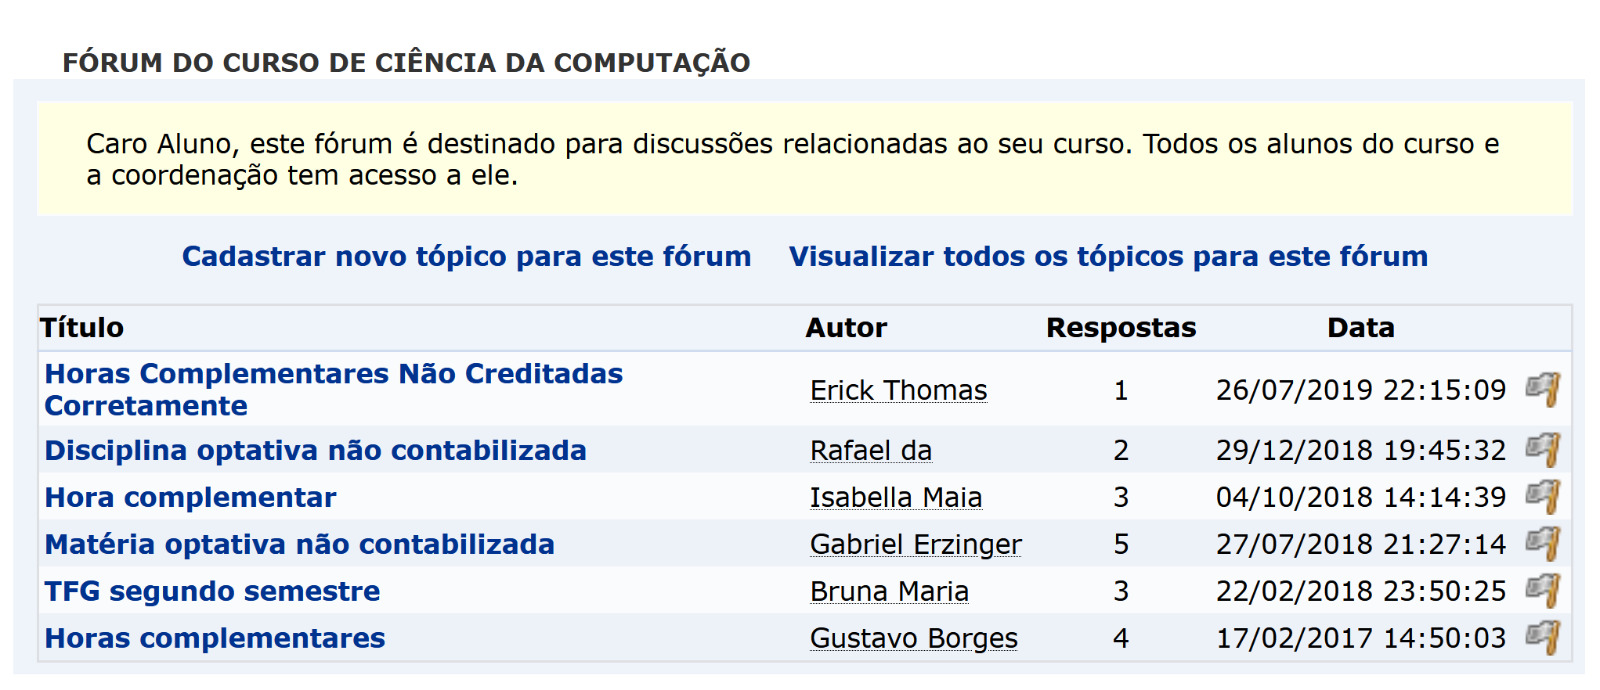
\includegraphics[width=\columnwidth]{figs/forum-sigaa-curso.png}
\caption{Fórum geral do curso de Ciência da Computação no SIGAA, com últimos tópicos de 2019.}
\label{fig-forum-curso}
\textit{\scriptsize Fonte: SIGAA UNIFEI (2026).}
\end{figure}

O padrão se repete nas demais instituições analisadas. A USP utiliza o e-Disciplinas, baseado no Moodle, sem ferramenta dedicada à discussão acadêmica; a UFMG combina o Moodle no UFMG Virtual com o sistema Siga, restrito a funcionalidades administrativas \citep{sigaufmg2019}; a UNESPAR adota o Moodle com o SIGES, voltado a solicitações burocráticas. Em todos os casos, o sistema acadêmico foi projetado para a gestão, e o ambiente de ensino, para a distribuição de conteúdo. A conversa ficou sem dono.

Parte da explicação está no desenho dessas ferramentas. \citet{bates2015} defende que o fórum não deve ser tratado como complemento do conteúdo, e sim como meio de construção do conhecimento, no qual os próprios alunos buscam recursos para fundamentar suas contribuições — o que exige recursos que sustentem a participação, e não apenas um espaço em branco onde publicar.

A base teórica dessa aposta vem da Teoria da Aprendizagem Social de \citet{bandura1977}, segundo a qual as pessoas aprendem comportamentos e atitudes observando umas às outras. Quando os alunos discutem, explicam e defendem ideias entre si, o esforço de organizar o raciocínio para apresentá-lo ao colega produz compreensão mais profunda do conteúdo. \citet{scager2016} acrescentam uma condição a isso: a aprendizagem colaborativa se torna efetiva quando existe interdependência positiva, ou seja, quando cada participante percebe que a sua contribuição é necessária ao resultado do grupo. Reunir alunos em torno de uma tarefa, por si só, não basta.

O Stack Overflow ilustra o que um ambiente projetado para essa finalidade consegue produzir: os usuários publicam dúvidas, outros respondem e a comunidade vota nas melhores respostas, que ganham destaque permanente \citep{vasilescu2014}. No contexto universitário, muitos alunos já improvisam algo semelhante no Discord, com servidores organizados por disciplina e canais para dúvidas e materiais. A demanda existe, portanto. O que falta é vínculo institucional, permanência do registro e diferenciação de papéis entre aluno, monitor e professor — sem a qual não há moderação possível nem forma de identificar a resposta confiável.

\subsection{Voluntariado Universitário}

O voluntariado contribui para a formação do estudante em duas frentes: desenvolve habilidades práticas, como liderança e trabalho em equipe, e constrói consciência social por meio do envolvimento com a comunidade. \citet{lopesjr2023} mostra, a partir de 259 respondentes, que a adesão cresce de maneira significativa quando a instituição se envolve ativamente — não basta disponibilizar os projetos.

Na UNIFEI, as ações de ONGs ligadas à extensão e as campanhas da atlética são divulgadas sobretudo no Instagram, sem plataforma que as centralize. O SIGAA possui um módulo de Ações de Extensão, apresentado na Figura \ref{fig-sigaa-extensao}, mas ele foi construído para a gestão administrativa: a tela de busca traz mais de quinze filtros institucionais, como Área do CNPq, Centro da Ação, Edital, Programa Estratégico, Dimensão Acadêmica e Unidade Proponente. São parâmetros úteis a uma pró-reitoria e inúteis a quem procura uma vaga compatível com o próprio curso. O módulo tampouco oferece inscrição direta ou comunicação com o coordenador do projeto.

\begin{figure}[!ht]
\centering
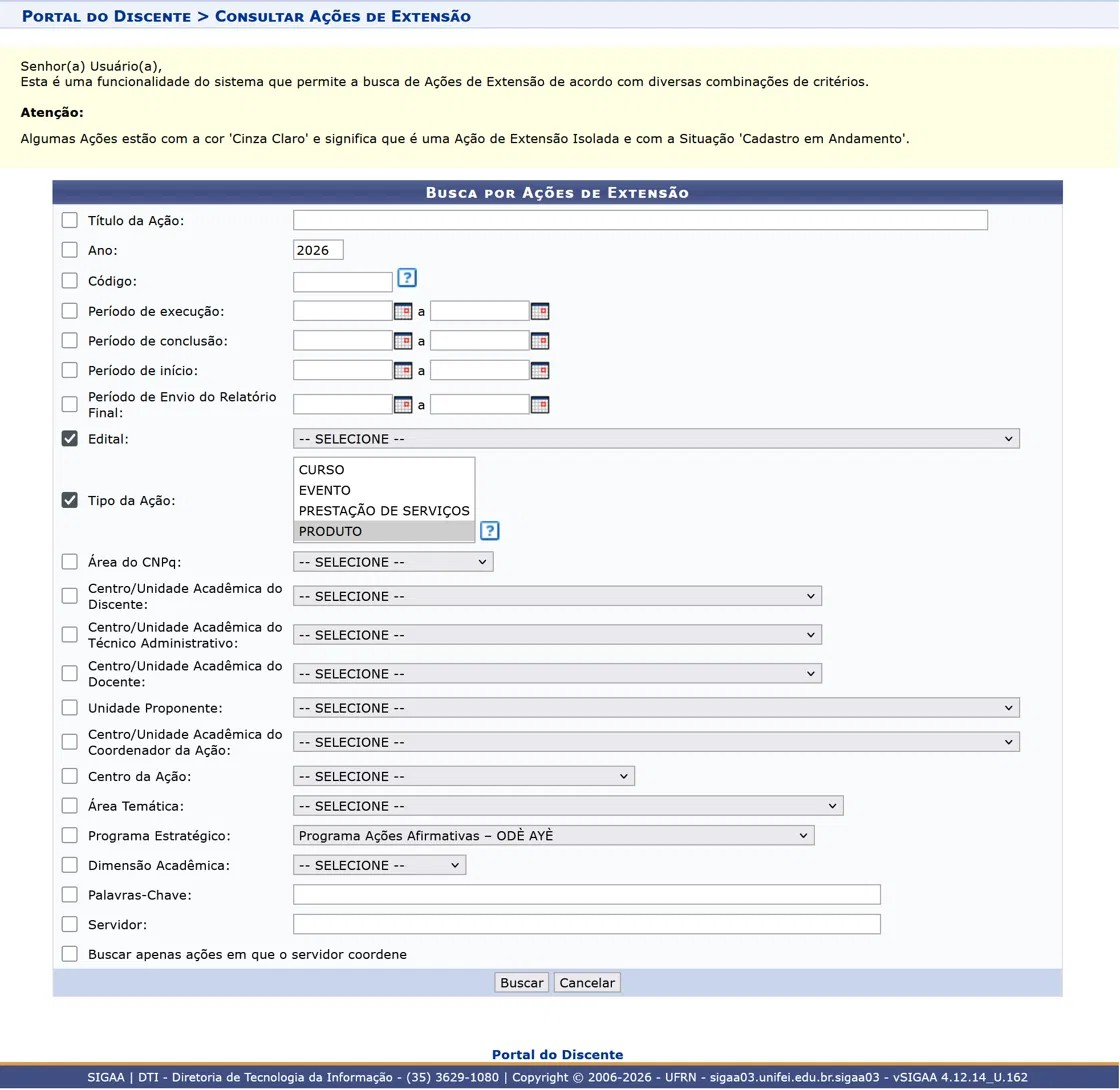
\includegraphics[width=\columnwidth]{figs/sigaa-extensao-busca.jpeg}
\caption{Tela de busca do módulo de Ações de Extensão do SIGAA da UNIFEI, com filtros voltados à gestão administrativa.}
\label{fig-sigaa-extensao}
\textit{\scriptsize Fonte: SIGAA UNIFEI (2026).}
\end{figure}

As outras instituições esbarram em limitações equivalentes. A UFMG mantém o SIEX, sistema de cadastro e gerenciamento de projetos de extensão, que permite consultar as atividades registradas mas não funciona como espaço no qual o aluno encontra oportunidades e se inscreve. Na UNESPAR, o registro das horas passa pelo SIGES em forma de solicitação burocrática, com o aluno selecionando manualmente a categoria do seu curso em um formulário, sem qualquer função de busca ou inscrição.

O custo dessa dispersão aparece depois que a atividade termina. Na UNIFEI, o coordenador solicita a emissão dos certificados à PROEX informando a matrícula de cada participante; em seguida, o próprio aluno pede o registro das horas no histórico, anexando o comprovante para que a coordenação do curso analise e aceite. São três etapas manuais para uma única participação, e o processo se repete de forma semelhante nas demais universidades analisadas. Como as atividades de extensão integram a grade curricular, a ausência de um fluxo que ligue inscrição, confirmação, certificado e registro de horas deixa de ser inconveniência administrativa e passa a ser obstáculo à própria integralização do curso.

\subsection{Análise Comparativa}

A Tabela \ref{tab-comparativo} sintetiza o levantamento, confrontando as funcionalidades oferecidas pelas plataformas das quatro instituições nos dois eixos examinados.

\begin{table}[!ht]
\centering
\caption{Comparativo entre as plataformas acadêmicas das universidades analisadas.}
\label{tab-comparativo}
\scriptsize
\begin{tabular}{|l|c|c|c|c|}
\hline
\textbf{Funcionalidade} & \textbf{UNIFEI} & \textbf{USP} & \textbf{UFMG} & \textbf{UNESPAR} \\
\hline
Sistema acadêmico & SIGAA & Júpiter & Siga & SIGES \\
\hline
Plataforma de ensino & Moodle & e-Disc. & Moodle & Moodle \\
\hline
Fórum disponível & Básico & Básico & Básico & Básico \\
\hline
Fórum efetivamente usado & Não & Não & Não & Não \\
\hline
Perfis por disciplina & Não & Não & Não & Não \\
\hline
Melhor resposta & Não & Não & Não & Não \\
\hline
Busca nos tópicos & Não & Não & Não & Não \\
\hline
Trabalho em grupo & Não & Não & Não & Não \\
\hline
Notificações em tempo real & Não & Não & Não & Não \\
\hline
Gestão de voluntariado & Ações Ext. & Não & SIEX & Não \\
\hline
Inscrição online & Não & Não & Não & Não \\
\hline
Registro de participação & Manual & Manual & Manual & Manual \\
\hline
Certificação integrada & Não & Não & Não & Não \\
\hline
\end{tabular}
\\ \vspace{5pt}
\textit{\scriptsize Fonte: Elaborado pela autora (2026).}
\end{table}

Nenhuma das instituições reúne, em um mesmo ambiente, um fórum com recursos que sustentem a participação e um sistema de voluntariado com inscrição, registro de horas e certificação automática. Os fóruns existem e não são usados; o voluntariado é gerido de forma descentralizada ou meramente burocrática; e o trabalho em grupo, que ocupa parte considerável da carga das disciplinas, não aparece em nenhuma das plataformas.

\subsection{Tecnologias Web}

Na camada de apresentação foram adotados o React.js, o TypeScript e o TailwindCSS. O React.js constrói interfaces a partir de componentes reutilizáveis, o que evita a repetição de um mesmo elemento em várias telas e facilita a manutenção conforme o projeto cresce \citep{react2024}. A escolha diante do Angular e do Vue.js considerou a curva de aprendizado, a maturidade do ecossistema e a presença da tecnologia no mercado brasileiro. O TypeScript acrescenta tipagem estática ao JavaScript, antecipando para o momento da escrita erros que só apareceriam em execução, e o TailwindCSS aplica estilo por classes utilitárias diretamente nos componentes, dispensando arquivos de estilo separados.

Na camada de aplicação, o Python com o framework Django oferece autenticação, painel administrativo, mapeamento objeto-relacional e proteções nativas contra ataques comuns, como CSRF (\textit{Cross-Site Request Forgery}) e injeção de SQL \citep{django2024}. O Django REST Framework organiza a construção da API por meio de serializadores e ViewSets, reduzindo código repetido nas operações de criação, leitura, atualização e remoção.

A comunicação em tempo real exigiu o protocolo WebSocket. No HTTP convencional, o cliente precisa consultar o servidor periodicamente para saber se algo mudou, prática conhecida como \textit{polling}; o WebSocket mantém uma conexão aberta e permite que a mensagem parta de qualquer um dos lados no instante em que o evento ocorre. A integração se dá pelo Django Channels \citep{channels2024}, que adiciona suporte ao protocolo ASGI (\textit{Asynchronous Server Gateway Interface}), com o Daphne como servidor de aplicação e o Redis como \textit{channel layer}, responsável por distribuir as mensagens entre as conexões.

O armazenamento ficou a cargo do PostgreSQL, banco relacional de código aberto que sustenta consultas complexas e oferece recursos como indexação textual e, por meio da extensão pgvector, busca por similaridade vetorial \citep{postgresql2024}. O Redis cumpre dois papéis: além do \textit{channel layer}, guarda os tokens de autenticação, dados de vida curta e escrita frequente que se beneficiam de um armazenamento em memória e que não precisam ocupar o banco relacional.
